
\subsection*{Aparatos PET}

 Una de las aplicaciones más importantes de la tecnología de detectores de física nuclear y de partículas a la imagen médica son los llamados aparatos PET, de las siglas en inglés Tomografía de Emisión de Positrones. Su principio de operación se basa en inyectar en el paciente un radiofármaco emisor de positrones, tal como la Fluordesoxiglucosa (18FDG), un azúcar radioactivo en el que un átomo de oxígeno se sustituye por uno de fluor-18 (\ensuremath{^{18}}F). El 18FDG se concentra en aquellas zonas del paciente que consumen elevadas cantidades de glucosa y por lo tanto puede actuar como trazador de procesos oncológicos (ya que las células tumorales son ávidas consumidoras de glucosa) así como de zonas del organismo con gran actividad metabólica, tales como el cerebro. El \ensuremath{^{18}}F se desintegra emitiendo un positrón, el cual se aniquila, tras un corto recorrido, con un electrón del tejido del paciente produciendo dos fotones de 511 kilo electrón voltios (keV) que se emiten en direcciones opuestas. 


%\begin{figure}
%\centering
\begin{center} \figbox[label={fig.PET}]{{\small Principio de operación del PET.}}{
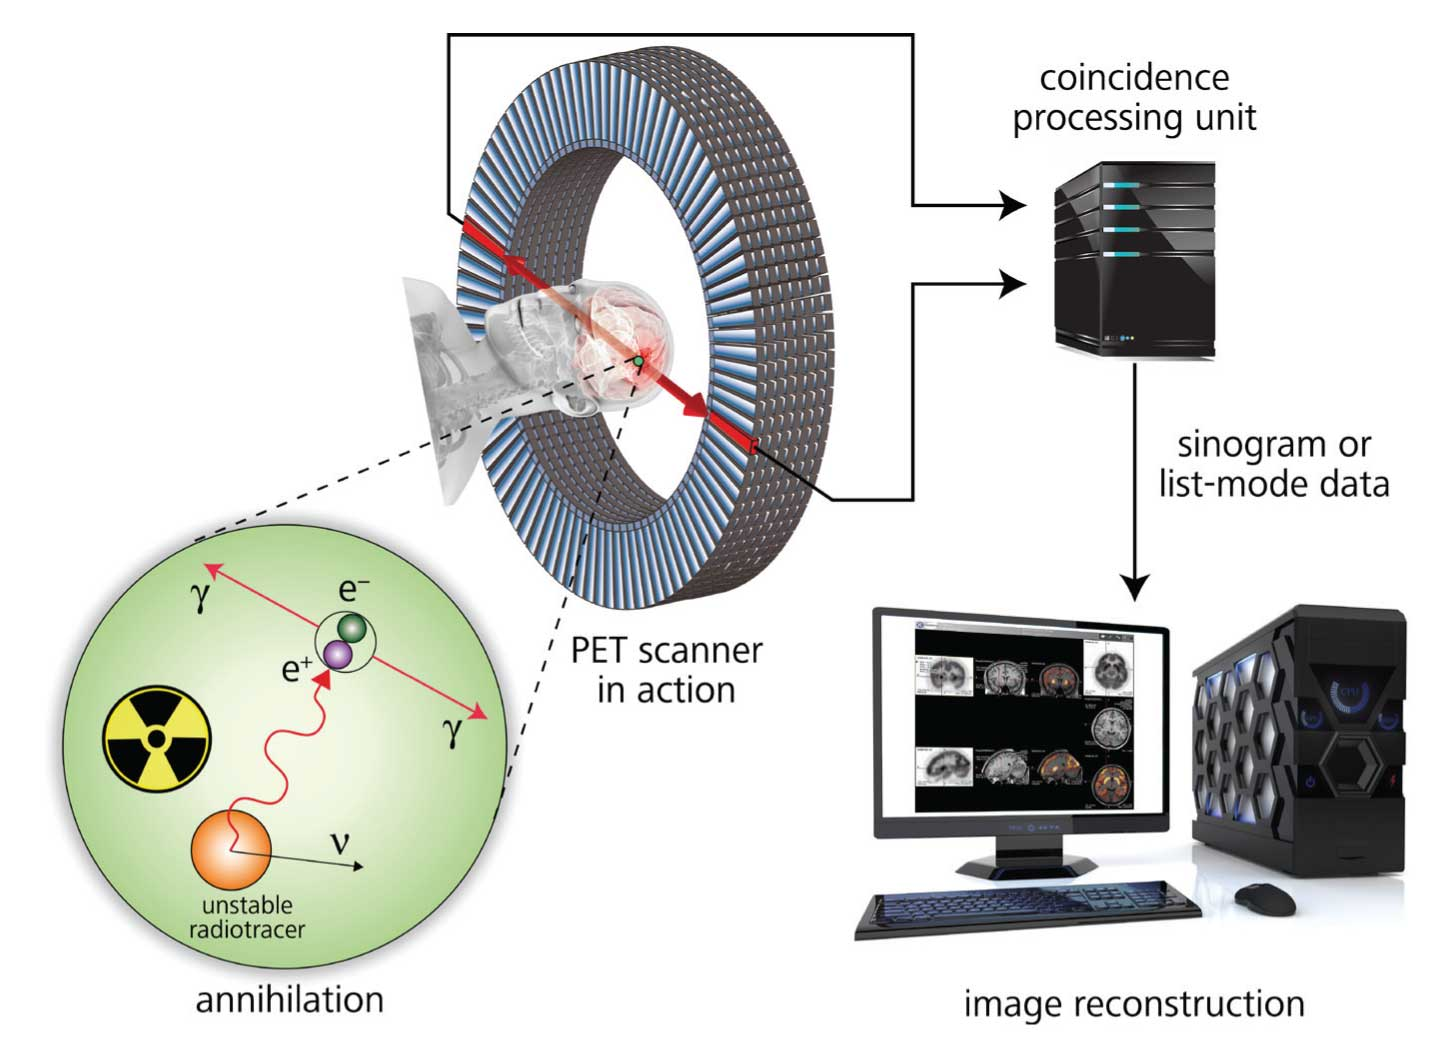
\includegraphics[width=0.6\textwidth]{img/PET.jpg}
%\caption{\small Principio de operación del PET.}
%\label{fig.PET}
} \end{center} 


Un PET clínico se construye a partir de varios anillos de detectores que rodean una determinada zona del cuerpo del paciente. Los fotones de 511 keV interaccionan con los detectores que forman el anillo, depositando su energía en ellos. Los detectores reconstruyen tanto la energía de los fotones originales como su punto de impacto. Puesto que los fotones se emiten en direcciones opuestas, cuando un par de detectores enfrentado entre sí en el anillo detectan interacciones simultáneas (dentro de la resolución temporal del sistema), pueden utilizarse los dos puntos de impacto reconstruidos para trazar una línea recta (o LOR, de las siglas en inglés de Línea de Respuesta) que pasa por el punto donde se aniquila el positrón con el electrón (el cual a su vez está muy próximo al punto de emisión del positrón). La intersección de muchas de estas LOR permite la reconstrucción funcional de la imagen (esto es, la reconstrucción de la zona en términos de su actividad metabólica), tal como se ilustra en la Figura \ref{fig.PET}.

El concepto de PET fue introducido a finales de la década de 1950 y la investigación básica que llevó a su implantación como aparato de imagen médica se ha seguido desarrollando a lo largo de las últimas seis décadas. Los aparatos PET de diseño moderno, basados en múltiples anillos de detectores, se desarrollan a partir de la década de 1990 y con mayor importancia a partir de los primeros años de la década de los 2000. Los aparatos originales utilizaban cristales ioduro de sodio (NaI) como material centelleador y PMTs como detectores de la luz visible emitida por estos cristales como respuesta a la interacción de los fotones de 511 keV. Durante los últimos cinco años, el campo ha experimentado una transformación importante, prefiriéndose en la actualidad los detectores de LSO o LYSO (de las siglas en inglés de Lutetium oxyorthosilicate o Lutetium-yttrium oxyorthosilicate) y un nuevo tipo de fotosensores llamados fotomultiplicadores de silicio (SiPMs de sus siglas en inglés). 

Los modernos aparatos PET basados en LYSO y SiPMs presentan muchas ventajas. El LYSO es un material muy denso (7.4 g/cm$^3$) capaz de detener a los fotones de 511 keV con una longitud de atenuación típica de 11 mm. Se trata además de un excelente centelleador que emite unos 14,000 fotones de luz azul (con un pico a 428 nm) por cada fotón de 511 keV absorbido. La copiosa emisión de luz se traduce a su vez en buena resolución en energía (del orden de 10-15 \% FWHM) y buena resolución espacial en la reconstrucción de las coordenadas transversas (con respecto a la dirección de vuelo) del punto de impacto (del orden de 1-3 mm) El tiempo de emisión es rápido, con una constante de atenuación de 40 ns, lo que permite una buena resolución en la coincidencia temporal (CRT de sus siglas en inglés) del orden de varios centenares de picosegundos en los sistemas comerciales más avanzados disponibles en la actualidad, tales como el GEMINI de Philips\footnote{http://www.healthcare.philips.com/main/products/nuclearmedicine/products/geminitf/}. Reducir el CRT tanto como sea posible es uno de los objetivos más importantes de la investigación actual en PET, ya que un CRT suficientemente bueno permite una mejora espectacular en la sensibilidad del sistema (la sensibilidad mide la calidad de la imagen que puede obtenerse por unidad de dosis absorbida en el paciente).  De hecho, la sensibilidad efectiva de un sistema PET para reconstruir un objeto de radio D mejora como D/CRT. 

Por otra parte, los sistemas basados en LYSO tienen algunos inconvenientes importantes. El mayor es el elevado precio de estos cristales, que a su vez constituye casi la mitad del coste del sistema PET. Un aparato comercial basado en LYSO puede costar hoy en día varios millones de euros. Este elevado coste, comparado con otras técnicas (tomografía axial, por ejemplo) limita el rango de aplicación del PET a la imagen médica. Por otra parte, las aplicaciones TOF de sistemas basados en LYSO, aunque posibles, están limitadas por la velocidad de centelleo intrínseca del centelleador (40 ns), el elevado índice de refracción (1.8)  y el hecho de que estos sistemas no miden en general la coordenada longitudinal (a lo largo de la línea de vuelo del fotón de 511 keV). Por tanto no se dispone de la medida de la profundidad de la interacción (DOI de sus siglas en inglés), lo que también limita la precisión en TOF. A pesar de estas limitaciones, el desarrollo de aparatos comerciales como el GEMINI de Philips, capaz de explotar la técnica TOF para mejorar su sensibilidad, a pesar de un modesto CRT (del orden de 500-600 ps), pone de manifiesto el extraordinario potencial de la tecnología.

\subsection*{Aplicación de la tecnología de Xenon Líquido a PET}

La posibilidad de construir un detector PET basado en el xenón líquido (LXe) fue propuesta por Chepel en 1973\footnote{Chepel, V.Y., 1993, Nucl. Tracks Radiat. Meas. 21, 47.}  pero la I+D+i subsiguiente se encontró con problemas tecnológicos que han limitado hasta la actualidad el desarrollo de este tipo de detectores\footnote{F. Nishikido et al. J. Appl. Phys. 43, 779 (2004).}. En concreto, la posibilidad de desarrollar un PET basado únicamente en la medida de la luz de centelleo del xenón fue estudiado hace una década por el grupo de Waseda, que obtuvo resultados modestos asociados a limitaciones tecnológicas, en concreto el uso de PMTs que a su vez limitaba la homogeneidad y hermeticidad de la celda de detección. 

No obstante, las propiedades físicas del LXe le permiten competir con ventaja con los mejores detectores de centelleo sólido, tales como el LYSO. Concretamente, el LXe produce el doble de luz (30,000 fotones) por fotón de 511 keV absorbido que el LYSO y una fracción importante de estos fotones (del orden de 6,000) se emiten con una constante de decaimiento muy rápida (2.2 ns). Por otra parte, la resolución temporal intrínseca de un sistema viene determinada por el número de fotones sobre la constante de decaimiento (N/$\tau$). N$/\tau$ =2,727 para la constante rápida ($\tau$ = 2.2~ ns) del LXe a comparar con N/$\tau$ =333 para el LYSO ($\tau$ = 40~ ns). Por tanto, el LXe proporciona, a priori, un CRT ocho veces mejor que el del LYSO. Pero además un detector basado en el LXe puede medir con precisión del orden de 1 mm las 3 coordenadas del punto de interacción del fotón incidente, mientras que la resolución en el DOI suele estar limitada en LYSO a varios milímetros. Por otra parte, la corrección en el tiempo de vuelo del fotón desde que se emite hasta que alcanza el fotodetector es importante (en el caso del LYSO esta corrección es aún más importante que en el LXe debido a su alto índice de refracción, 1.8 a comparar con 1.55), lo que implica una mayor degradación del CRT en LYSO comparado con LXe. Como consecuencia, el LXe ofrece la posibilidad de construir un detector PET con una resolución CRT muy superior a la del LYSO. La resolución intrínseca de la celda centelleadora de xenón líquido, LXSC  se ha calculado en 20 ps\footnote{J.J. Gómez-Cadenas, charla plenaria en la conferencia CSI 2015, artículo en preparación (proceedings, CSI 2015). }  lo que permite la posibilidad de construir sistemas comerciales con un CRT un orden de magnitud mejor de los que obtiene el sistema GEMINI. Un sistema de este tipo supondría una auténtica revolución en la tecnología PET.

La segunda característica de interés del LXe es su bajo coste, del orden de un factor 5 inferior (por unidad de detección) al LSYO. Esto permite la posibilidad de construir un PET que conjunte una sensibilidad muy superior a los modelos convencionales (gracias a la aplicación TOF) con un coste sensiblemente inferior. 

%\begin{figure}
%\centering
\begin{center} \figbox[label={fig.BOX}]{{\small Diseño de la LXSC.}}{
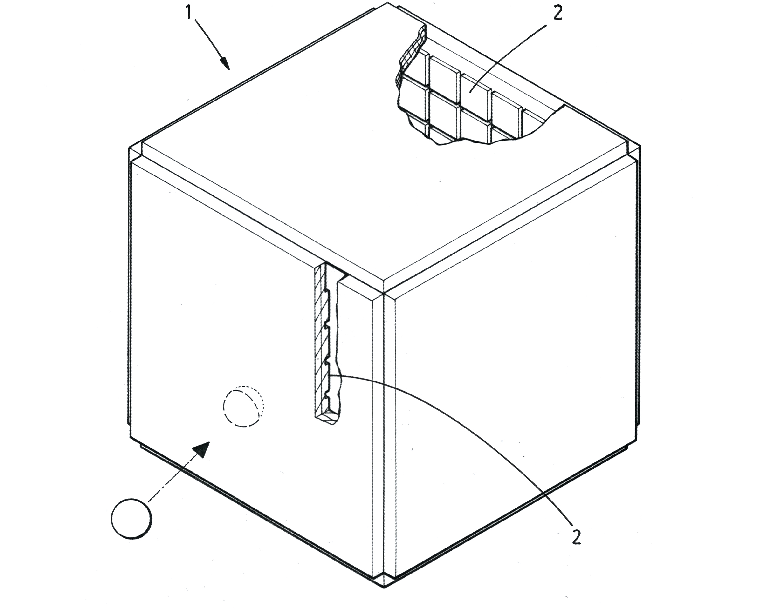
\includegraphics[width=0.6\textwidth]{img/LXSC2.pdf}
%\caption{\small Diseño de la LXSC.}
%\label{fig.BOX}
} \end{center} 

Por otra parte, la propuesta, la celda centelladora de xenón líquido (LXSC)\footnote{Celda centelleadora de LXe, patente número P201531239 presentada en 31 agosto 2015 ante la OPEM (MINECO), CSIC/UV, inventor J.J. Gómez-Cadenas.} resuelve los problemas tecnológicos encontrados por los pioneros de esta técnica, tales como el grupo de Waseda. El modelo estándar de LXSC es una caja de $5\times 5 \times 5$~ cm$^3$ (las dimensiones y la forma pueden variar dependiendo de la aplicación) rellena de LXe (Figura \ref{fig.BOX}). Cuatro de las 6 superficies internas de la LXSC están recubiertas por una lámina de teflón que refleja con 95\% de eficiencia la luz UV (172 nm) emitida por el xenón. La cara de entrada y salida (con respecto a la dirección de vuelo de los fotones) están recubiertas por SiPMs sensibles a la luz UV (fabricados en la actualidad por Hamamatsu y a cuyo desarrollo han contribuido de forma muy importante miembros del GI). El tamaño de los SiPMs puede ajustarse según la aplicación y el coste del dispositivo, variando típicamente entre 3 mm y 6 mm de lado. La LXSC ofrece una buena resolución en energía (del orden del 12 \% FWHM), buena resolución espacial (1 mm) en las tres coordenadas y excelente CRT\footnote{J.M. Benlloch Rodríguez, tesis de Master, Universidad de Valencia, 2015, dirigida por J.J. Gómez-Cadenas. 
}. {\bf Es posible, por lo tanto, construir en la comunidad valenciana un nuevo tipo de sistema PET basado en la LXSC que suponga, a la vez, una mejora en las prestaciones y una reducción del coste, relativo a los sistemas actuales.}
\subsection*{Objetivos: PETALO}

El segundo objetivo de este proyecto es realizar contribuciones esenciales para el desarrollo del proyecto PETALO, necesarias para demostrar su viabilidad y para evaluar sus capacidades. Los objetivos específicos son los siguientes: i) medida de ciertas propiedades físicas del LXe, cruciales para aplicaciones PET;  ii) caracterización de la resolución de energía y la resolución espacial de la LXSC; medida de la resolución de coincidencia temporal (CRT de sus siglas en inglés) de la LXSC.

\subsubsection*{Medida de las propiedades físicas de LXe}
La resolución en energía, resolución espacial y CRT del LXe depende de la cantidad total de fotones de centelleo ultravioleta (UV) producidos como respuesta a los fotones de 511 keV característicos del PET. Depende también de la fracción de la energía depositada que resulta en centelleo y en ionización. Son necesarias, por tanto, las siguientes medidas:
\begin{itemize}
\item El número total de fotones UV producidos como respuesta a fotones de 511 keV. 
\item Fracción de fotones UV debida a centelleo primario y fracción debida a la recombinación lenta de los electrones de ionización. 
\item Fracción de fotones UV debida al modo singlete y su constante de centelleo.
\item Fracción de fotones UV debida al modo triplete y su constante de centelleo. 
\end{itemize}

\subsubsection*{Medida de la resolución en energía y resolución espacial de la LXSC}

La resolución en energía de un detector de centelleo de xenón líquido es una combinación de varios factores, a saber: factor debido a la geometría del detector R$_g$, debido a la fluctuación estadística de los fotoelectrones en los sensores R$_s$, y fluctuación intrínseca, R$_i$, debida a las fluctuaciones que introducen los electrones que no se recombinan y la no proporcionalidad de la luz de centelleo:

\begin{equation}
\mathrm{R}^2 = \mathrm{R}_g^2 + \mathrm{R}_s^2 +  \mathrm{R}_i^2
\end{equation}

Este proyecto propone una medida experimental de R. La contribución de 
R$_g$~y R$_s$~se puede obtener mediante un cálculo Monte Carlo y a partir de ahí determinar la contribución intrínseca. Se espera obtener una resolución de 12\% FWHM competitiva con la de centelladores como LSO/LYSO. 

La resolución espacial en las coordenadas (x,y) se obtendrá a partir de algoritmos de baricentro que pesan la posición de los SiPMs con la amplitud del pulso. La resolución en la coordenada longitudinal se obtendrá a partir del cociente entre la amplitud total registrada en el plano de entrada y en el de salida. Se espera obtener una resolución del orden de 1--2 mm FWHM en las tres coordenadas.     

\subsubsection*{Medida de la resolución temporal de la LXSC}

La resolución temporal (CRT) de la LXSC depende de dos factores: a) la resolución temporal asociada con el disparo (trigger) de una interacción en una LXSC y b) la fluctuación temporal introducida por la sincronización de diferentes celdas.

La resolución temporal asociada a una LXSC o resolución intrínseca del sistema (ya que la resolución de sincronización, puede, en principio, reducirse arbitrariamente mediante la electrónica adecuada) depende a su vez de varios factores, a saber: el cociente $N/\tau$, donde $N$~es el número de photons emitidos con una constante temporal dada $\tau$; b) la corrección longitudinal o corrección de profundidad de interacción (DOI) que toma en cuenta el hecho de que no todas las interacciones ocurren en el mismo punto; c) la función de respuesta a fotones (PDE) de los SiPM; d) la fluctuación temporal introducida por los SiPMs y su electrónica asociada. 

El número esperado de fotones en LXe con una constante rápida (2.2 ns) es del orden de 6,000, por tanto  $N\tau$ = 6,000/2.2 = 2,727, a comparar con el correspondiente número para LSO $N\tau$ = 14,000/40 = 35. Por tanto, la CRT intrínseca del LXe es mucho mejor que la del LSO.  Nuestros estudios preliminares sugieren la posibilidad que se pretende demostrar experimentalmente, de un CRT  mejor de 100 ps, incluyendo el efecto de los SiPMs y la electrónica. 

\subsubsection*{El detector P2}

%\begin{figure}
%\centering
\begin{center} \figbox[label={fig.P2}]{{\small Esquema del detector P2.}}{
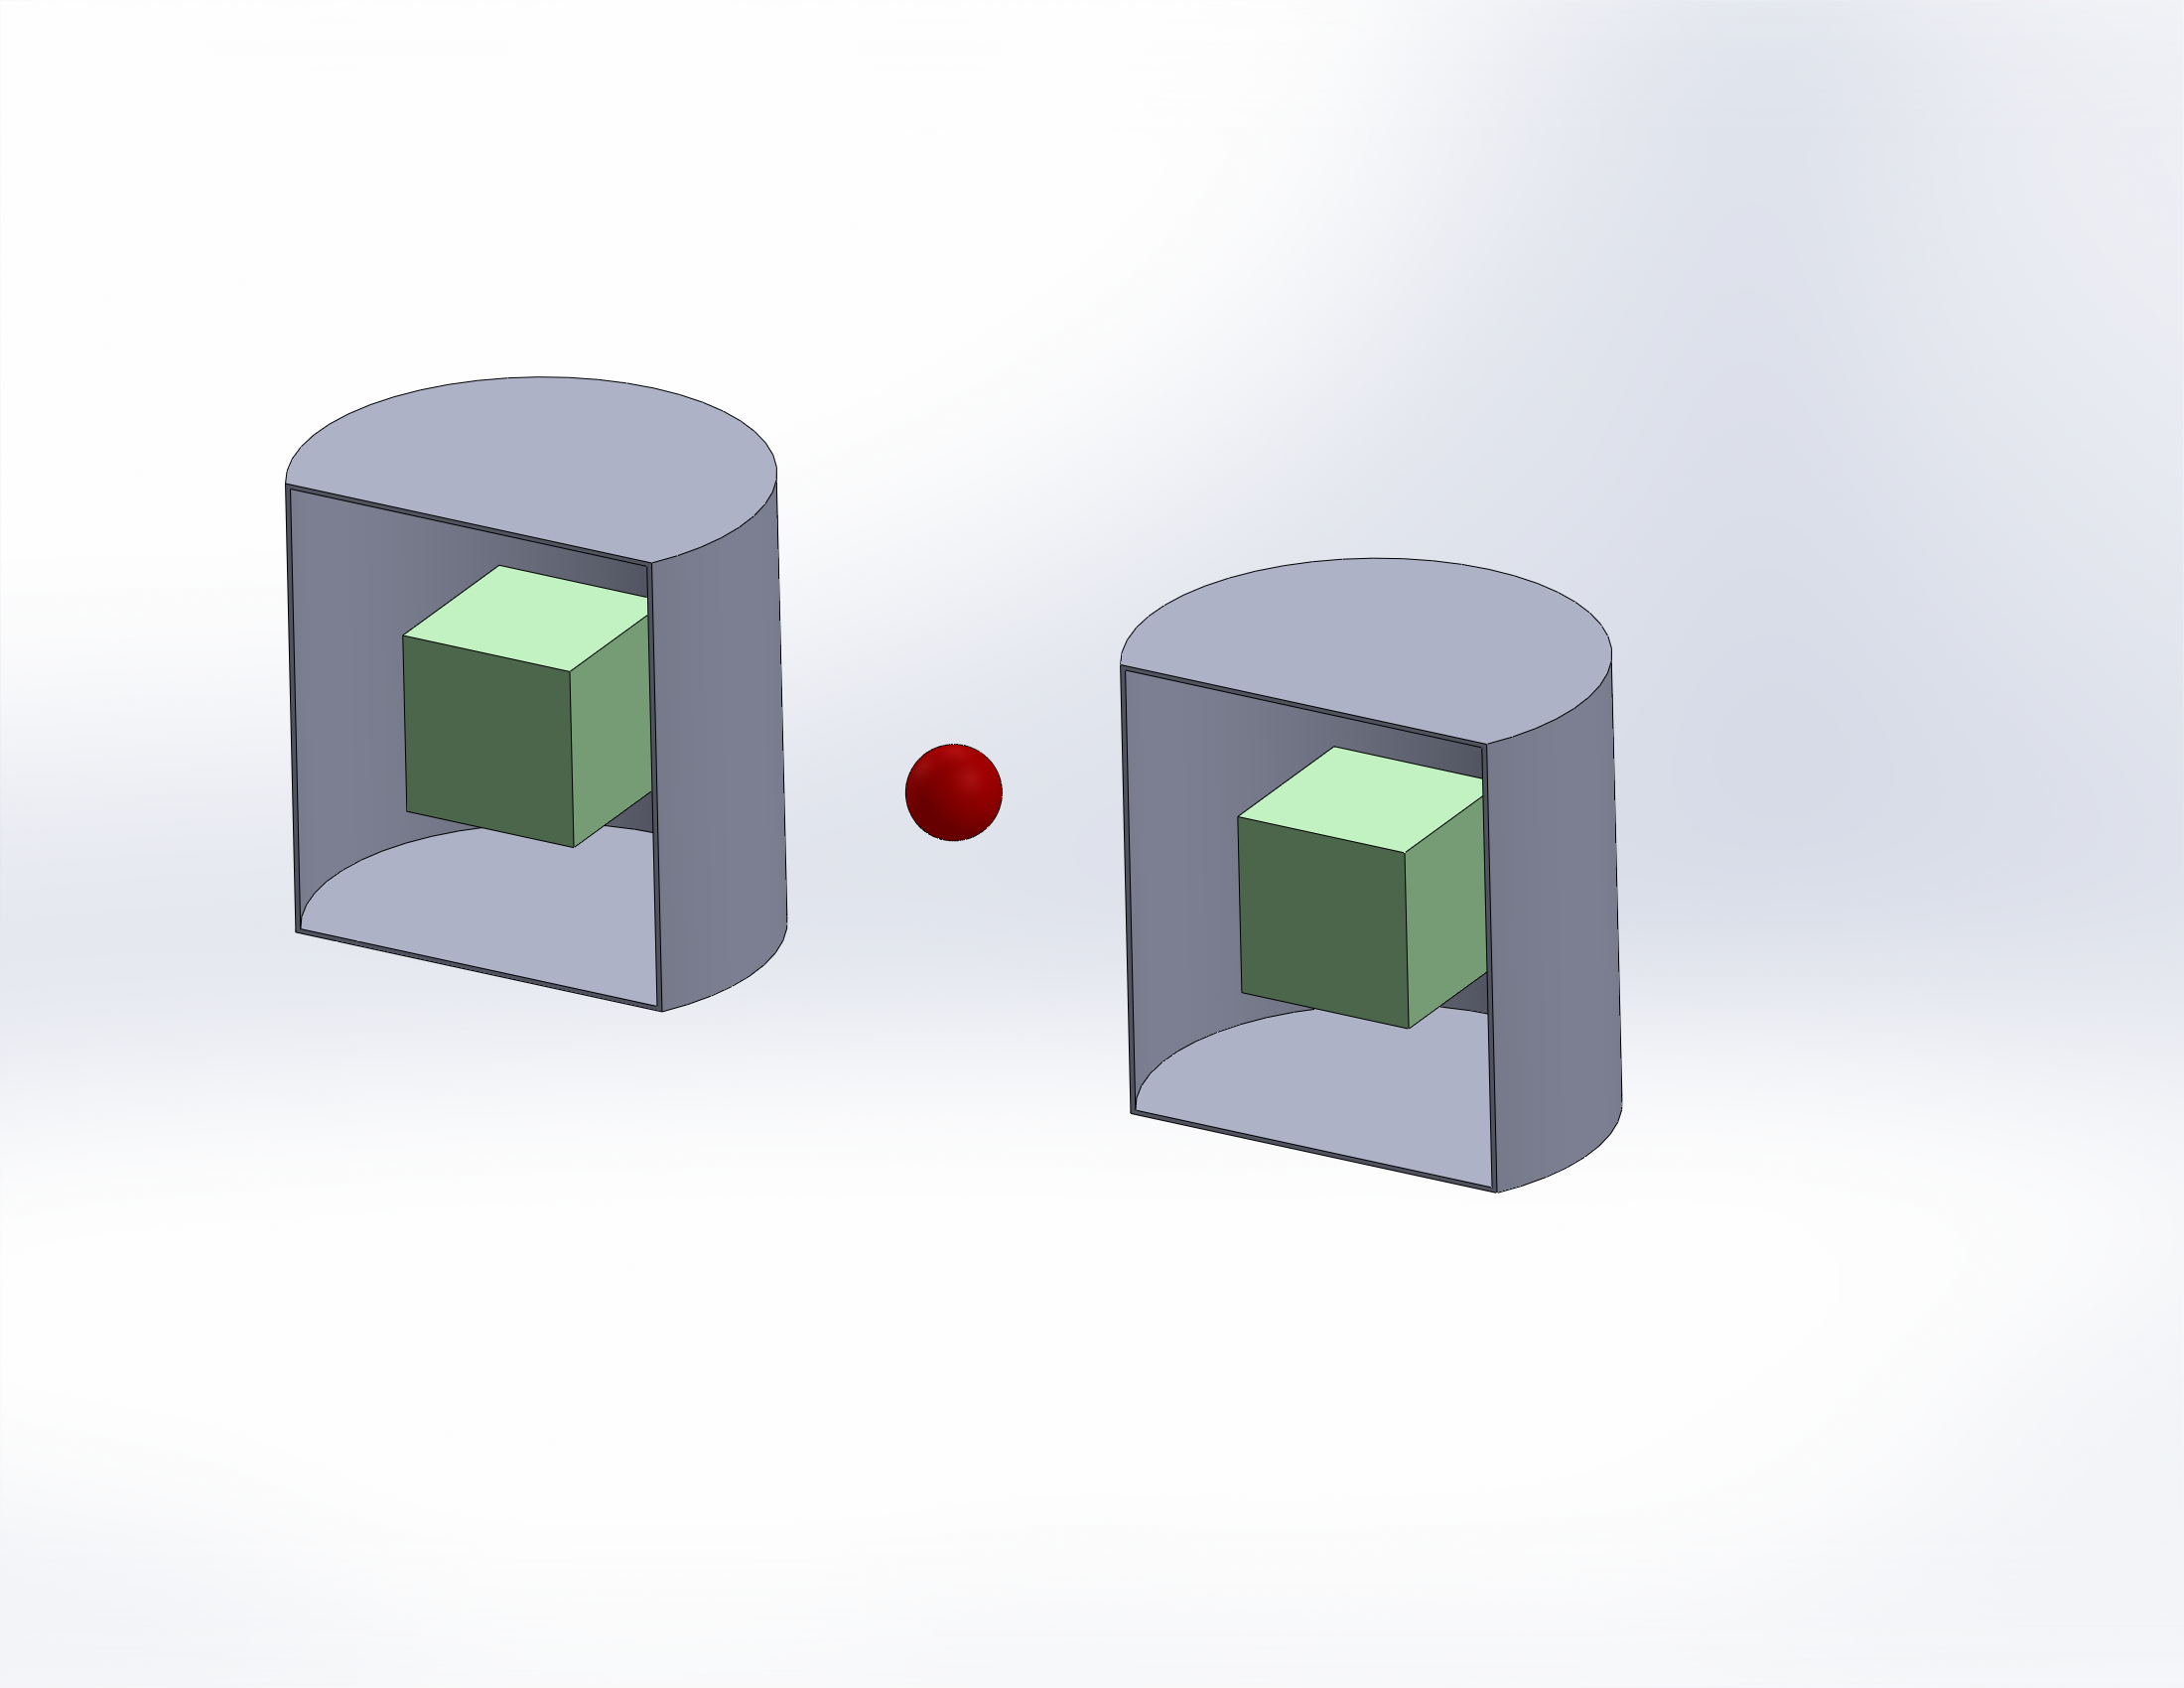
\includegraphics[width=0.6\textwidth]{img/P2.png}
%\caption{\small Esquema del detector P2.} 
%\label{fig.P2}
} \end{center}

La medida de la resolución espacial, resolución en energía y resolución CRT requiere la construcción de un sistema de test especializado que denominamos P2 (Figura \ref{fig.P2}). Se trata de dos LXSC independientes, cada una de las cuales está albergada en su propio criostato. Una de las LXSC (PA) tendrá todas las caras internas instrumentadas, a fin de poder utilizar la redundancia de las medidas de las coordenadas $(x,y)$, $(x,z)$, $(y,z)$ y la determinación independiente de la coordenada $z$~para medir la resolución en posición de la LXSC. Asímismo, la comparación de la resolución del primer fotoelectrón entre PA y la segunda LXSC (PB), que sólo tendrá dos caras instrumentadas, permitirá entender la influencia en el CRT del tiempo de tránsito de los fotones.  

\subsubsection*{Construcción y operación de un demostrador preclínico}
Una vez medidos los parámetros críticos de PETALO (resolución en energía, resolución espacial y CRT), se procederá a la construcción de un anillo constituido por catorce LXSC, que permita caracterizar la sensibilidad de un aparato PET-TOF basado en LXe. Para ello se utilizarán fantasmas estándar (NEMA phantoms) que permitirán medir los parámetros operacionales del escáner así como su fiabilidad a la hora de reconstruir imágenes.

\subsection*{Desarrollo del proyecto}
Las actividades a realizar en el proyecto PETALO durante los próximos cuatro años son:
\begin{enumerate}
\item {\bf 2016}: La construcción de un dispositivo experimental, basado en 2 LXSC cuya operación en coincidencia permite medir el CRT del sistema, así como la resolución en energía y resolución espacial de las celdas (P2).
\item {\bf 2017}: Operación de P2. Medidas de resolución y CRT. Construcción del criostato y la mecánica de un demostrador pre-clínico consistente en un anillo de 14 LXSC (PDEMO). 
\item {\bf 2018}: Construcción de los módulos de PDEMO. Puesta a punto y calibración. 
\item {\bf 2019}: Evaluación de la sensibilidad PDEMO y de su resolución TOF. Preparación de un proyecto para la construcción y comercialización de un PET-TOF de alta sensibilidad combinado con resonancia magnética (RMI) para neuroimagen cerebral.   
\end{enumerate}

\subsection*{Financiación del proyecto}

En este proyecto de investigación se solicita financiación para la construcción de P2 y de PDEMO así como para un ingeniero compartido con el proyecto NEXT. Por otra parte, el proyecto se beneficiará de la gran sinergia existente con el proyecto NEXT. En particular, PETALO utilizará el laboratorio de NEXT existente en el IFIC, así como las infraestructuras (sistema de gas, equipos de vacío, recuperación criogénica, sistema de test para SiPMs, etc.) lo que permitirá un abaratamiento muy considerable de los costes de desarrollo. 

%Sinergia entre NEXT y PETALO. 
%
%Como se ha expuesto más arriba, la tecnología que ha dado lugar al proyecto PETALO se ha derivado de la experiencia adquirida por el IP y el grupo de investigación en el desarrollo del proyecto NEXT. Concretamente, la celda centelladora de xenón líquido, LXSC, se instrumenta utilizando los KDBs desarrollados para NEXT.
%
%Un aspecto donde la sinergia entre ambos proyectos revierte desde PETALO hasta NEXT es la electrónica del plano de lectura. En el diseño original de NEXT, implementado en los detectores NEXT-DEMO y NEW, se utiliza electrónica discreta disponible comercialmente (COTS, de sus siglas en inglés). Dicha electrónica es fiable y proporciona una excelente respuesta, pero resulta muy cara, con un coste del orden de 150 euros por canal. De hecho, la electrónica del plano de trazado de NEXT-100 se presupuestó en cerca de 1 millón de euros. Dado lo ajustado de la financiación para el proyecto NEXT, reducir este coste es esencial para poder construir el detector final. 
%
%Por otra parte, ningún sistema PET que aspire a implantarse comercialmente puede permitirse electrónica COTS, dado su alto precio. La solución, sin embargo, ya ha existe en el ámbito PET, con el desarrollo de varios ASIC especializados para leer SiPMs, entre los que cabe destacar el TOFPET y TOFPET2 de PETSYS . Cada ASIC cuenta con 64 canales (por tanto puede adaptarse a un KDB) y su coste de producción es del orden de 20 € por canal. 
%
%Durante 2016, el proyecto PETALO pondrá en marcha el demostrador P2, utilizando el TOFPET, cuya resolución temporal es excelente. Como consecuencia, es posible certificar, en 2017, la viabilidad de una electrónica basada en ASIC (en lugar de en COTS) no sólo para PETALO, sino también para NEXT-100. Esta solución permitiría reducir el coste de la electrónica de NEXT-100 desde casi un millón de euros hasta 140,000 euros, lo que supondría un ahorro esencial para el proyecto. 
%
%
%
%
%
%
%

























